\documentclass[12pt]{article}
\usepackage[utf8]{inputenc}
\usepackage{pgfplots}
\usetikzlibrary{shapes.geometric, arrows}
\usetikzlibrary{automata}
\tikzstyle{bluenode} = [circle, minimum width=1cm, minimum height=1cm,text centered, draw=black, fill=blue!30]
\tikzstyle{rednode} = [circle, minimum width=1cm, minimum height=1cm,text centered, draw=black, fill=red!30]
\tikzstyle{brownnode} = [circle, minimum width=1cm, minimum height=1cm,text centered, draw=black, fill=brown!30]
\tikzstyle{arrow} = [thick,->,>=stealth]

\tikzstyle{startstop} = [ellipse, minimum width=3cm, text centered, draw=black, fill=yellow!30]
\tikzstyle{process} = [rectangle, rounded corners, minimum width=3cm, text centered, draw=black, text width=5cm, fill=blue!30]
\tikzstyle{decision} = [diamond,  minimum width=3cm, aspect=2.5, text centered, draw=black, fill=green!30]
\pgfplotsset{compat=1.18}
\author{Mahir Labib Dihan}
\title{My first LaTeX}
\begin{document}
\begin{center}
    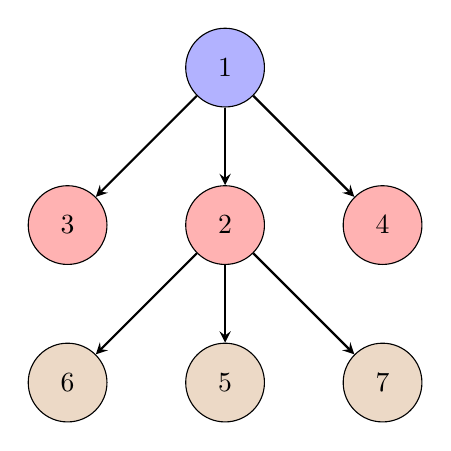
\begin{tikzpicture}[node distance=2cm]
        \node (node1) [bluenode] {1};
        \node (node2) [rednode, below of=node1] {2};
        \node (node3) [rednode, left of=node2] {3};
        \node (node4) [rednode, right of=node2] {4};

        \node (node5) [brownnode, below of=node2] {5};
        \node (node6) [brownnode, left of=node5] {6};
        \node (node7) [brownnode, right of=node5] {7};

        \draw [arrow] (node1) -- (node2);
        \draw [arrow] (node1) -- (node3);
        \draw [arrow] (node1) -- (node4);

        \draw [arrow] (node2) -- (node5);
        \draw [arrow] (node2) -- (node6);
        \draw [arrow] (node2) -- (node7);
    \end{tikzpicture}

\end{center}

\begin{center}
    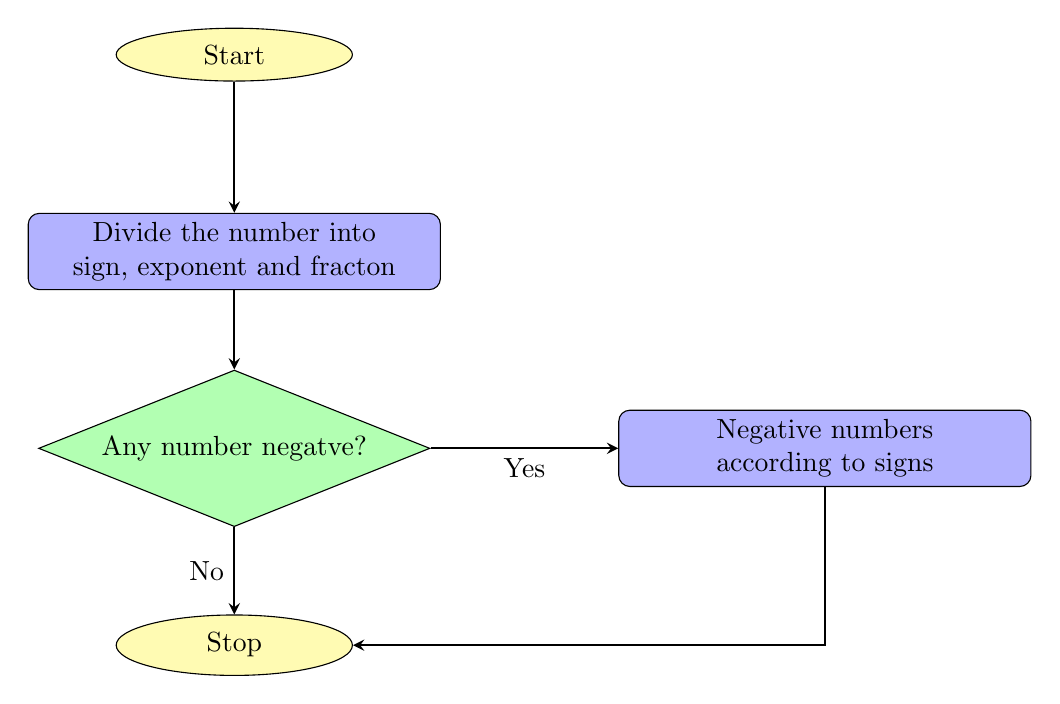
\begin{tikzpicture}[node distance=2.5cm]
        \node (start) [startstop] {Start};
        \node (pro1) [process, below of=start] {Divide the number into sign, exponent and fracton};
        \node (dec1) [decision, below of=pro1] {Any number negatve?};
        \node (pro2) [process, right of=dec1,xshift=5cm] {Negative numbers according to signs};
        \node (stop) [startstop, below of=dec1] {Stop};
        \draw [arrow] (start) -- (pro1);
        \draw [arrow] (pro1) -- (dec1);
        \draw [arrow] (dec1) -- (stop) node[midway, left] {No};
        \draw [arrow] (dec1) --  (pro2) node[midway, below] {Yes};
        \draw [arrow] (pro2) |- (stop);
    \end{tikzpicture}
\end{center}

\begin{center}
    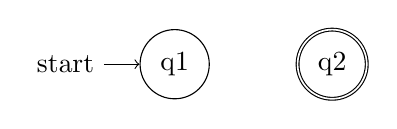
\begin{tikzpicture}[node distance=2cm]
        \node (A) [initial,state] {q1};
        \node (B) [accepting,state, right of=A] {q2};
    \end{tikzpicture}
\end{center}
\end{document}